\section{System Architecture}
\label{sec:sd-architecture}

The structure diagrams follow the building block view of arc42, equivalent to the context, container and component levels of the C4 model; together with the behavior, deployment and database diagrams they cover the views of the 4+1 model~\cite{kruchten1995}.

\subsection{Building Blocks}
\label{sec:sd-building-blocks}

\begin{figure}[H]
    \centering
    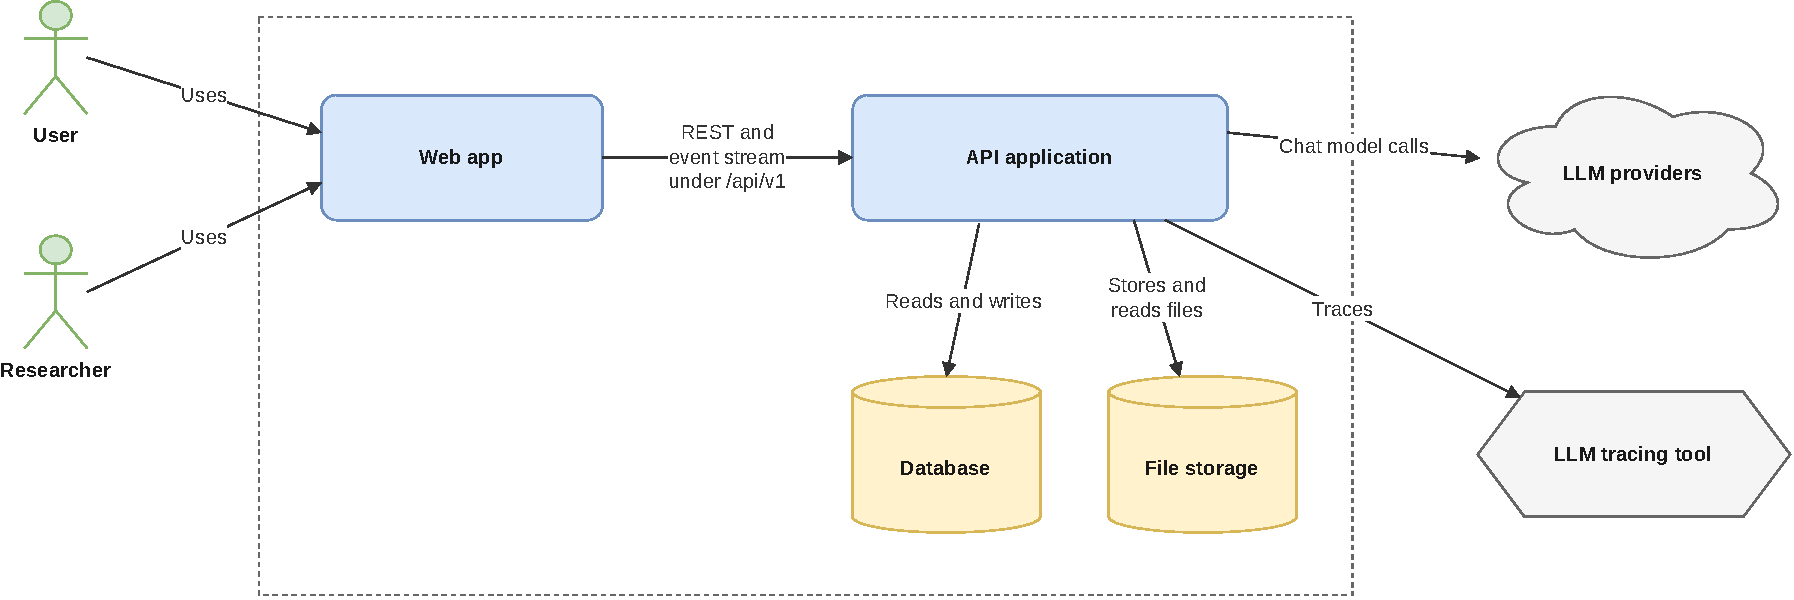
\includegraphics[width=\linewidth]{system-design/building-blocks.pdf}
    \caption{Building blocks of the system.}
    \label{fig:sd-building-blocks}
\end{figure}

\begin{itemize}
    \item \textbf{Web app}: chat, workflow graph, artifact panel and settings. It holds no business logic and draws the workflow and the artifacts from data the API provides.
    \item \textbf{API application}: REST and event stream API, authentication, execution of the agent workflow as background tasks, calls to the LLM providers.
    \item \textbf{Database}: application data, run events, workflow checkpoints and vectors.
    \item \textbf{File storage}: exported documents and uploaded files.
\end{itemize}
The workflow writes its events to an event log in the database and the stream endpoint reads the log; the workflow never writes into an HTTP response, so a closed browser does not stop a run and a reconnecting client gets the events it missed.

\subsection{Backend Modules}
\label{sec:sd-backend-modules}
The API application is one deployable unit, a modular monolith. Figure~\ref{fig:sd-backend-modules} shows its modules and the allowed import directions.

\begin{figure}[H]
    \centering
    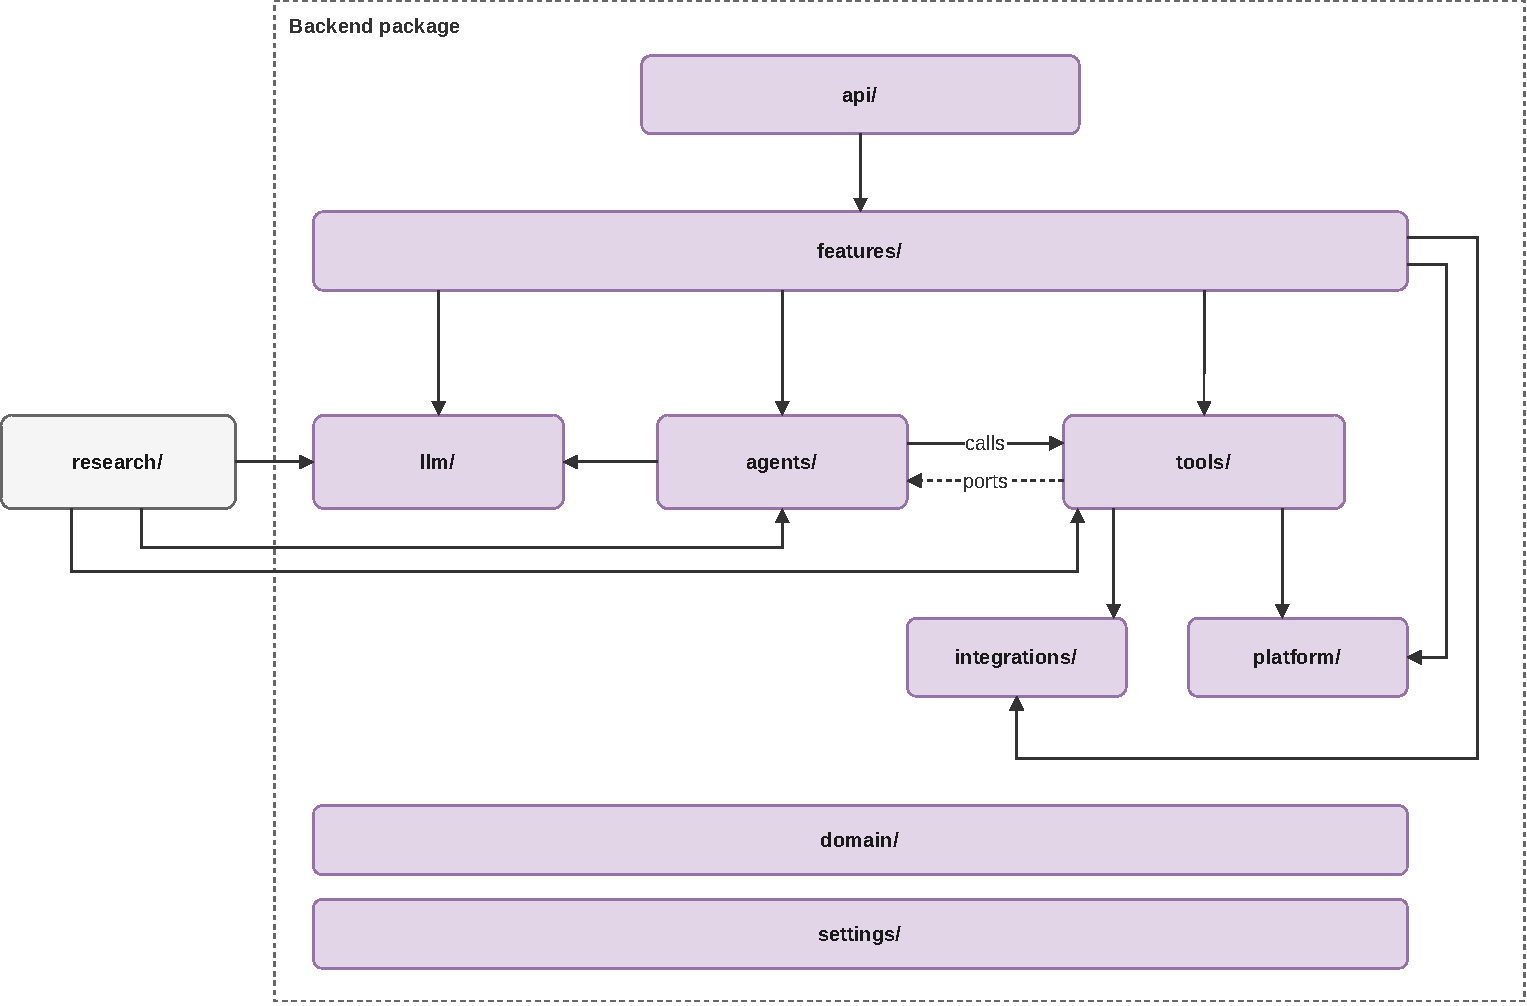
\includegraphics[width=0.85\linewidth]{system-design/backend-modules.pdf}
    \caption{Backend modules and allowed import directions.}
    \label{fig:sd-backend-modules}
\end{figure}

\begin{table}[H]
    \centering
    \caption{Responsibilities of the backend modules.}
    \label{tab:sd-backend-modules}
    \begin{tabularx}{\linewidth}{|l|X|}
        \hline
        \textbf{Module} & \textbf{Responsibility} \\
        \hline
        \texttt{api/} & Mounts the feature routers under \texttt{/api/v1}; maps domain errors to HTTP responses \\
        \texttt{features/} & One package per business feature (auth, projects, threads, runs, artifacts, model settings), each with a router, schemas, a service, a repository and models \\
        \texttt{agents/} & The workflow graph: state, nodes, prompts, ports, and the versioned workflow definition \\
        \texttt{llm/} & The only place that creates chat models; resolves an agent role to a provider and a model; checks cost limits and records usage around every call \\
        \texttt{tools/} & Tools that agents can call, such as research search \\
        \texttt{platform/} & Database session, object storage client, background run executor \\
        \texttt{domain/} & Business rules without infrastructure: content schemas, integrity rules, domain errors \\
        \texttt{settings/} & Application settings and logging \\
        \texttt{research/} & Evaluation harness, outside the backend, importing the same agents \\
        \hline
    \end{tabularx}
\end{table}

\subsection{Frontend Architecture}
\label{sec:sd-frontend}

\begin{figure}[H]
    \centering
    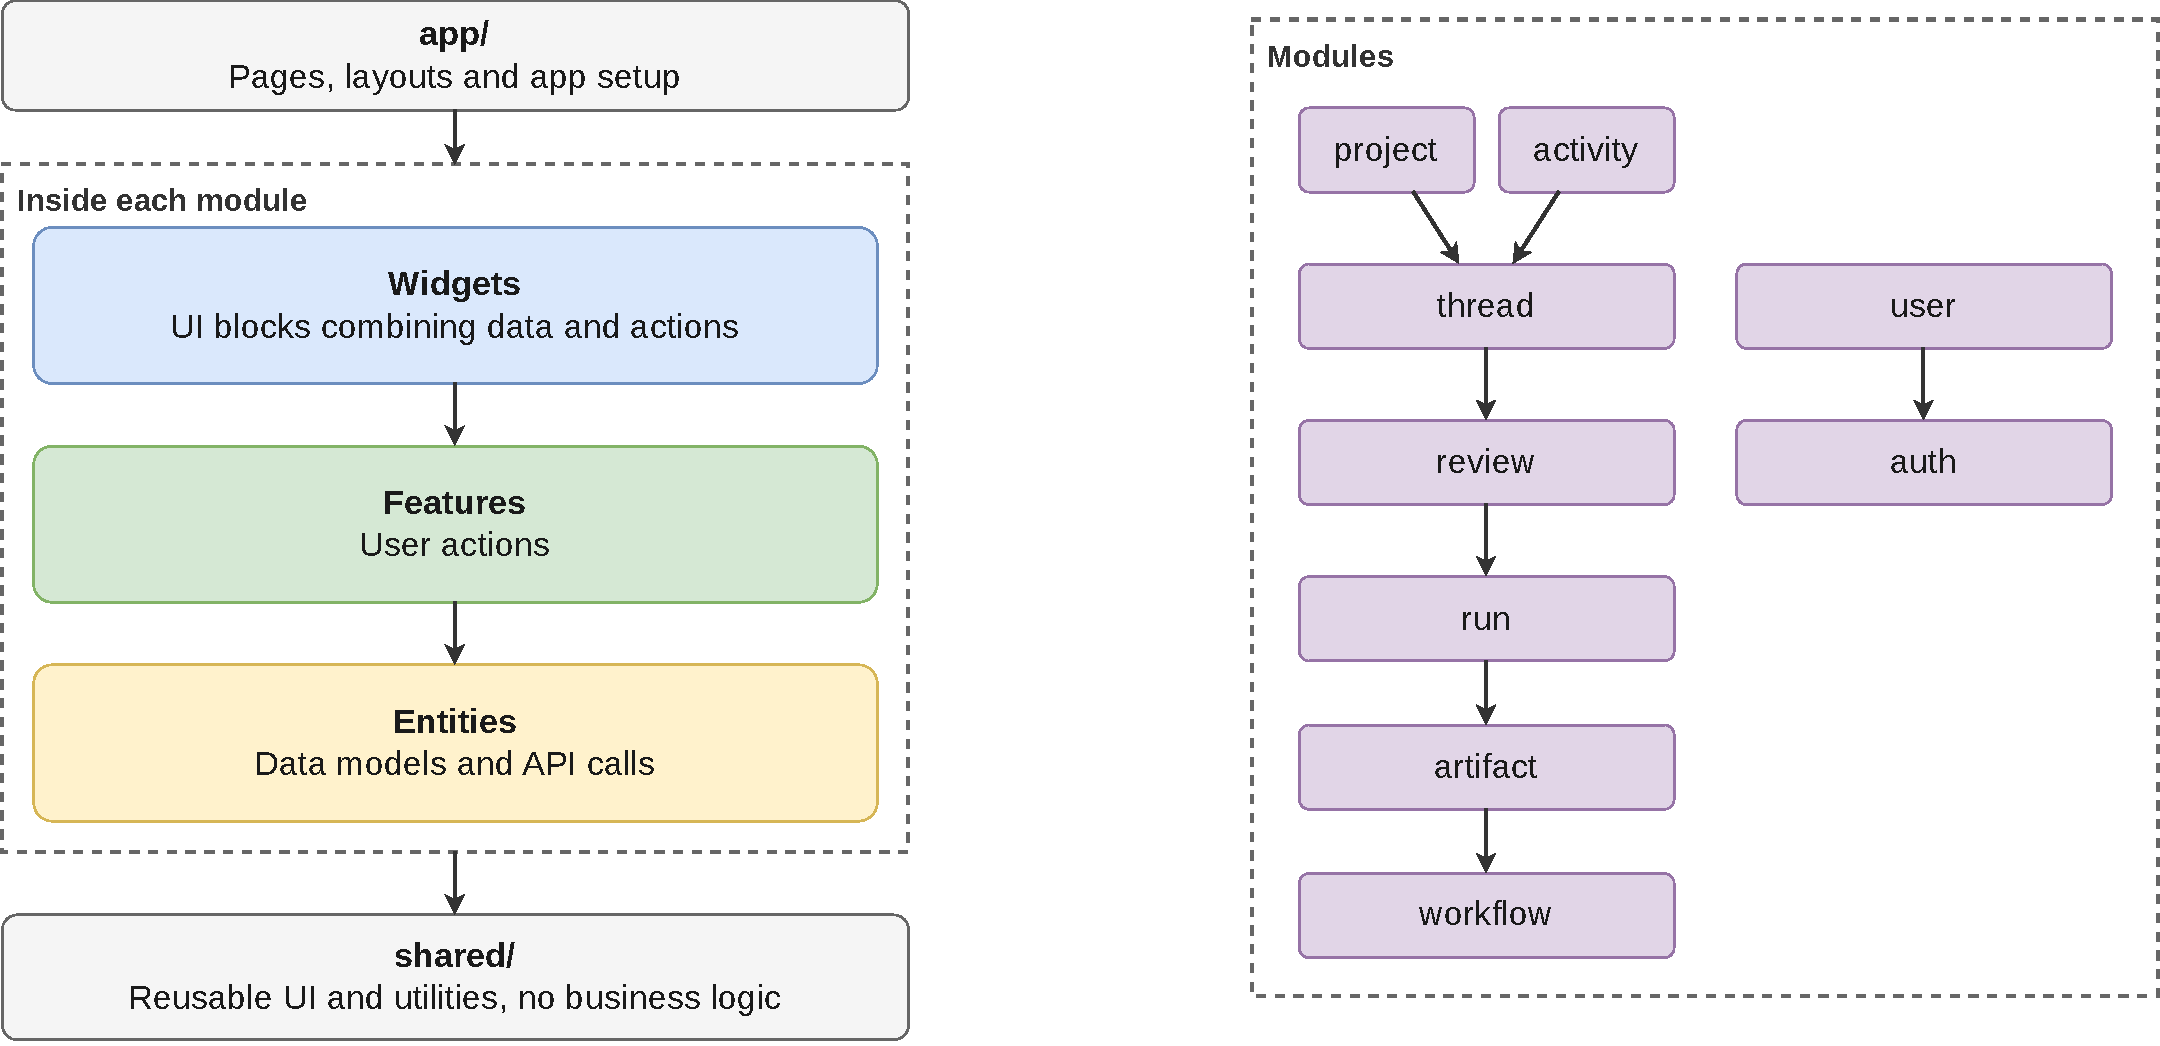
\includegraphics[width=\linewidth]{system-design/frontend-architecture.pdf}
    \caption{Frontend architecture.}
    \label{fig:sd-frontend}
\end{figure}
\todo{Describe the layers of the web app: routes, features, typed API client generated from the OpenAPI schema, server state and client state.}

\subsection{Deployment}
\label{sec:sd-deployment}

\begin{figure}[H]
    \centering
    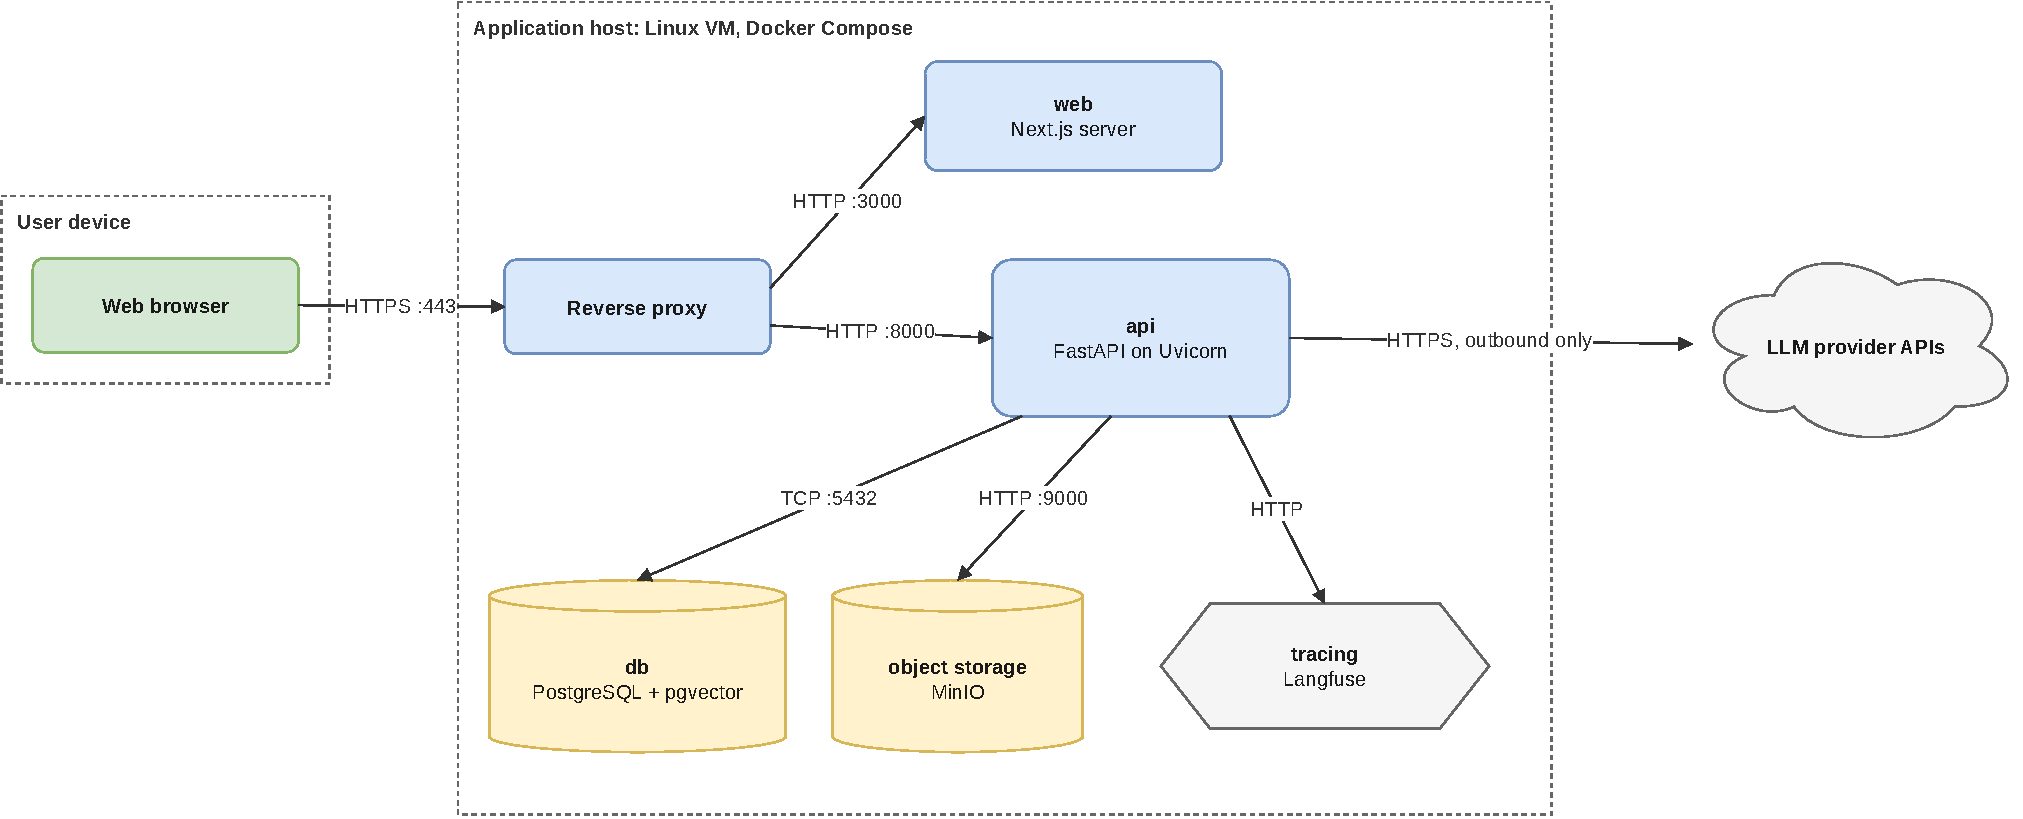
\includegraphics[width=\linewidth]{system-design/deployment-production.pdf}
    \caption{Deployment diagram (production).}
    \label{fig:sd-deployment}
\end{figure}
\todo{Describe the nodes (reverse proxy, web, api, db, object storage, tracing) and the constraints: same origin, one API process, long-lived responses.}
